\documentclass[lang=cn,11pt,a4paper]{elegantpaper}

% Rerun LaTeX compilation process
% to resolve the "Rerun to get /PageLabels entry" error.
% You may need to run LaTeX multiple times until the error is resolved.
\date{\zhtoday}
\title{课程作业}
\usepackage{array}
\newcommand{\ccr}[1]{\makecell{{\color{#1}\rule{1cm}{1cm}}}}
\definecolor{shadecolor}{RGB}{241, 241, 255}
\newcounter{problemname}
\newenvironment{problem}{\begin{shaded}\stepcounter{problemname}\par\noindent\textbf{题目\arabic{problemname}. }}{\end{shaded}\par}
\newenvironment{solution}{\par\noindent\textbf{解答. }}{\par}
\begin{document}
\maketitle
\section{题目}
仍考虑例1.1中的问题,但现在假设猪的价格保持稳定,设\begin{align}
    p = 0.65 - 0.01t +0.00004t^2
\end{align}表示t天后猪的价格(美分/磅).
\subsection{(a)}
1.画图:
\begin{figure}[h]
    \centering
    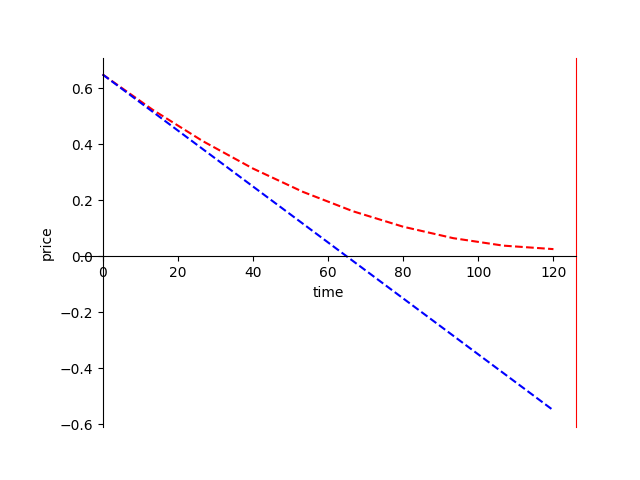
\includegraphics[width=0.5\linewidth]{1.png}
    \caption{价格图像}
    \label{价格图像}
\end{figure}
根据图像可知:他们在\(t=0\)处的图像接近.
\subsection{(b)}
五步方法:1.提出问题:同例题1.1
2.选择建模方法:我们选择单变量优化模型.3.推导模型的公式:
\begin{align*}
    Q=(0.65 - 0.01x +0.00004x^2)(200+5x)-0.45x
\end{align*}
4.求解模型:
\begin{align*}
    f^{'}(x)=\frac{3X^2 -420x +4000}{5000} 
\end{align*}
经过求解可得:\(f^{'}\)的零点取值为\(x= 70 \pm \frac{10\sqrt{321}}{3} \approx 10.28 \text{et} 129.72\) 
5.回答问题:
利润在10天之后达到顶点,最大利润值为129.72
\subsection{(c)}
设价格平稳率的参数\(a\)根据模型公式和导数运算可得:
\begin{align*}
    x &= -\frac{\sqrt{16000000a^2-12800a +1}+4000a -1}{300a} \\
    \frac{dx}{da} &= -\frac{\sqrt{16000000a^2 -12800a +1}+6400a -1}{300a^2\sqrt{16000000a^2 -12800a +1}}
\end{align*}
将\(a=0.00004\)代回可得:
\begin{align*}
    S(x,a) &= \frac{dx}{da} * \frac{a}{x} \\ 
    &=0.31
\end{align*}
如果价格提高比预期快10\% , 预期的售猪时间要增加3.1\% .
同样的:得到\(S(y,a) = 0.005\),如果价格提高比预期快10\%,预期的纯利润要增加0.05\%
\subsection{(d)}
由(c)中所展示的灵敏性来看,(b)中的最优解和例题中的最优解并没有极大差距,对价格的假设是稳健的
\end{document}